\documentclass[10pt]{beamer}
\usepackage{amsmath}
\usefonttheme{professionalfonts} % using non standard fonts for beamer
\usefonttheme{serif} % default family is serif\
\usepackage{mathtools}
%\documentclass[12pt]{beamerthemeSam.sty}
\usepackage{epsf}
\usepackage{ulem}
\usepackage{array}
%\usepackage{pstricks}
%\usepackage[orientation=portrait,size=A4]{beamerposter}
\geometry{paperwidth=160mm,paperheight=120mm}
%DT favorite definitions
\def\LL{\left\langle}   % left angle bracket
\def\RR{\right\rangle}  % right angle bracket
\def\LP{\left(}         % left parenthesis
\def\RP{\right)}        % right parenthesis
\def\LB{\left\{}        % left curly bracket
\def\RB{\right\}}       % right curly bracket
\def\PAR#1#2{ {{\partial #1}\over{\partial #2}} }
\def\PARTWO#1#2{ {{\partial^2 #1}\over{\partial #2}^2} }
\def\PARTWOMIX#1#2#3{ {{\partial^2 #1}\over{\partial #2 \partial #3}} }

\def\rightpartial{{\overrightarrow\partial}}
\def\leftpartial{{\overleftarrow\partial}}
\def\diffpartial{\buildrel\leftrightarrow\over\partial}

\def\BI{\begin{itemize}}
\def\EI{\end{itemize}}
\def\BE{\begin{displaymath}}
\def\EE{\end{displaymath}}
\def\BEA{\begin{eqnarray*}}
\def\EEA{\end{eqnarray*}}
\def\BNEA{\begin{eqnarray}}
\def\ENEA{\end{eqnarray}}
\def\EL{\nonumber\\}
\def\BS{\bigskip}
\def\BC{\begin{center}}
\def\EC{\end{center}}
\def\BCC{\begin{columns}}
\def\ECC{\end{columns}}
\def\HC{\column{0.5\textwidth}}
\newcommand{\etal}{{\it et al.}}
\newcommand{\gbeta}{6/g^2}
\newcommand{\la}[1]{\label{#1}}
\newcommand{\ie}{{\em i.e.\ }}
\newcommand{\eg}{{\em e.\,g.\ }}
\newcommand{\cf}{cf.\ }
\newcommand{\etc}{etc.\ }
\newcommand{\atantwo}{{\rm atan2}}
\newcommand{\Tr}{{\rm Tr}}
\newcommand{\dt}{\Delta t}
\newcommand{\op}{{\cal O}}
\newcommand{\msbar}{{\overline{\rm MS}}}
\def\chpt{\raise0.4ex\hbox{$\chi$}PT}
\def\schpt{S\raise0.4ex\hbox{$\chi$}PT}
\def\MeV{{\rm Me\!V}}
\def\GeV{{\rm Ge\!V}}

%AB: my color definitions
%\definecolor{mygarnet}{rgb}{0.445,0.184,0.215}
%\definecolor{mygold}{rgb}{0.848,0.848,0.098}
%\definecolor{myg2g}{rgb}{0.647,0.316,0.157}

\definecolor{A}{rgb}{0.8,0.0,0.0}
\definecolor{B}{rgb}{0.0,0.6,0.0}
\definecolor{C}{rgb}{0.4,0.4,0.0}
\definecolor{D}{rgb}{0.0,0.0,0.5}
\definecolor{E}{rgb}{0.4,0.4,0.4}


\definecolor{abtitlecolor}{rgb}{0.0,0.255,0.494}
\definecolor{absecondarycolor}{rgb}{0.0,0.416,0.804}
\definecolor{abprimarycolor}{rgb}{1.0,0.686,0.0}
\definecolor{Red}           {cmyk}{0,1,1,0}
\definecolor{Grey}           {cmyk}{.5,.5,.5,0}
\definecolor{Lg}           {cmyk}{.4,.4,.4,0}
\definecolor{Blue}          {cmyk}{1,1,0,0}
\definecolor{Green}         {cmyk}{1,0,1,0}
\definecolor{Brown}         {cmyk}{0,0.81,1,0.60}
\definecolor{Black}         {cmyk}{0,0,0,1}

\usetheme{Madrid}
\setbeamercolor{title}{fg=abtitlecolor}
\setbeamercolor{frametitle}{fg=abtitlecolor}
\setbeamercolor{palette tertiary}{fg=white,bg=abtitlecolor}
\setbeamercolor{palette secondary}{fg=white,bg=absecondarycolor}
\setbeamercolor{palette primary}{fg=black,bg=abprimarycolor}
\setbeamercolor{structure}{fg=abtitlecolor}

\setbeamerfont{section in toc}{series=\bfseries}

%AB: remove navigation icons
\beamertemplatenavigationsymbolsempty
\title{
  \textbf {Torque}\\
%\centerline{}
%\centering
%\vspace{-0.0in}
%\includegraphics[width=0.3\textwidth]{propvalues_0093.pdf}
%\vspace{-0.3in}\\
%\label{intrograph}
}

\author[W. Freeman] {Physics 211\\Syracuse University, Physics 211 Spring 2023\\Walter Freeman}

\date{\today}

\begin{document}

\frame{\titlepage}


%\frame{\frametitle{\textbf{Announcements}}
%\Large
%We are still grading Exam 3; we will get those back to you Friday.
%
%\BS
%
%Homework 8 will be posted later today or tomorrow morning; it will be due a week from Wednesday.
%
%\BS
%
%There will be a Homework 9, due to your TA's mailbox on the last day of class.
%
%\BS 
%
%Office hours this week: 
%
%\BI
%\item Thursday, 1:45-3:45
%\item Friday, 9:30-11:30
%\EI
%}
%
%\frame{\frametitle{\textbf{Agenda for today}}
%\Large
%
%We didn't quite finish the process-of-science discussion from Thursday.
%
%\BS
%
%After we finish that up, we'll start Unit 4.
%
%}
%
%
%
%\frame{\frametitle{\textbf{Statistical dishonesty}}
%\large
%{\color{Red}Statistics} is the mathematical discipline that lets us turn empirical data into conclusions.
%
%\BS
%
%It lets us turn a collection of ``maybes'' and ``probablys'' and ``unlikelys'' into ``almost certainlys''.
%
%\BS\BS
%
%\normalsize
%
%Statistics is immensely powerful. But:
%
%\BI
%\item It is a subtle, complex field of math (you can get PhD's in it)
%\item It is a lot of work and only someone intimately familiar with data is really equipped to analyze it
%\pause
%\item {\color{Red}It is absolutely essential if science is going to look to empirical data as the highest authority}
%\EI
%
%\BS
%\BS
%
%A great many flawed scientific processes come down to flawed statistics. Some common statistical fallacies:
%
%\normalsize
%\BI
%\item ``Garbage in, garbage out'': flawed, stinky data $\rightarrow$ statistical analysis $\rightarrow$ incorrect but nonstinky conclusions!
%\item Correlation implies causation
%\item Incorrect use of statistical inference (statistics is hard)
%{\color{Red}
%\item Some types of cherry-picking:
%\BI
%\item ``P-hacking''
%\item Publication bias
%\EI
%}
%\EI
%}
%
%\frame{\frametitle{\textbf{Statistical inference done honestly}}
%
%Suppose we want to test if a new drug (or a chemical in food) has any effect.
%
%\BS
%
%Correct thing to do:
%
%\BI
%\item Make lots of measurements of how people react to the drug
%\item Compare their distribution to the black curve (what you'd expect if the drug does nothing)
%\item Get excited if their average is very different from the center of the curve (maybe drug made that happen?)
%\BI
%\item (Statistics gives us tools to quantify ``very different'')
%\EI
%\EI
%
%
%\BC
%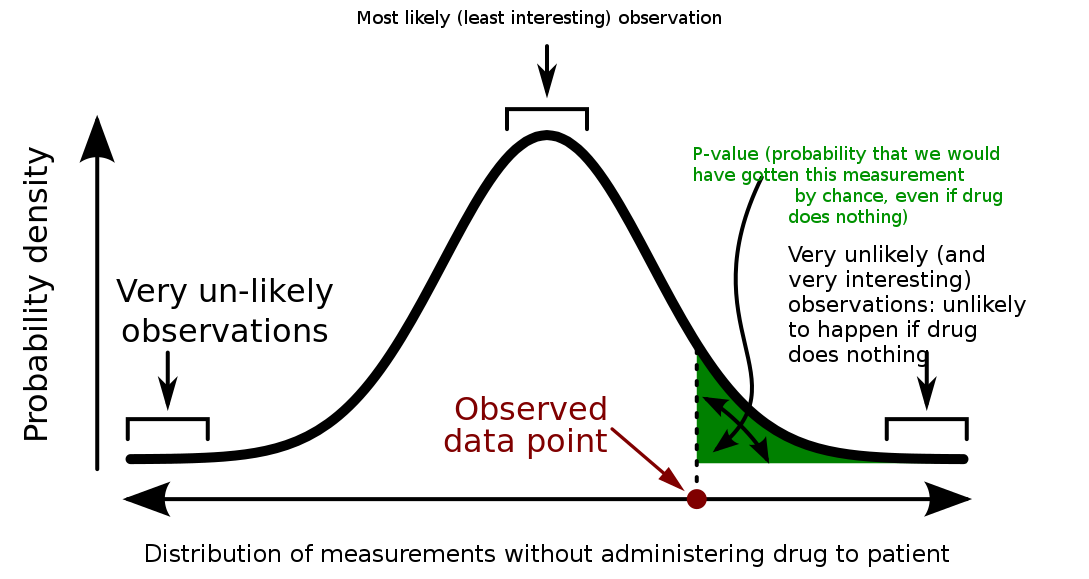
\includegraphics[width=0.8\textwidth]{gaussian.png}
%\EC
%}
%
%\frame{\frametitle{\textbf{Statistical inference gone wrong, I: cherry-picking}}
%
%\BS
%
%Classic cherry-picking:
%\BI
%\item Make lots of measurements of how people react to the drug
%\item {\color{Red} Forget about the ones close to the center (they are boring!)}
%\item Compare their distribution to the black curve (what you'd expect if the drug does nothing)
%\item {\color{Red} Even if the drug does nothing, you'll get a distribution looking like the green portion}
%\item {\color{Red} Notice that their average is very different, get excited!}
%\EI
%
%
%\BC
%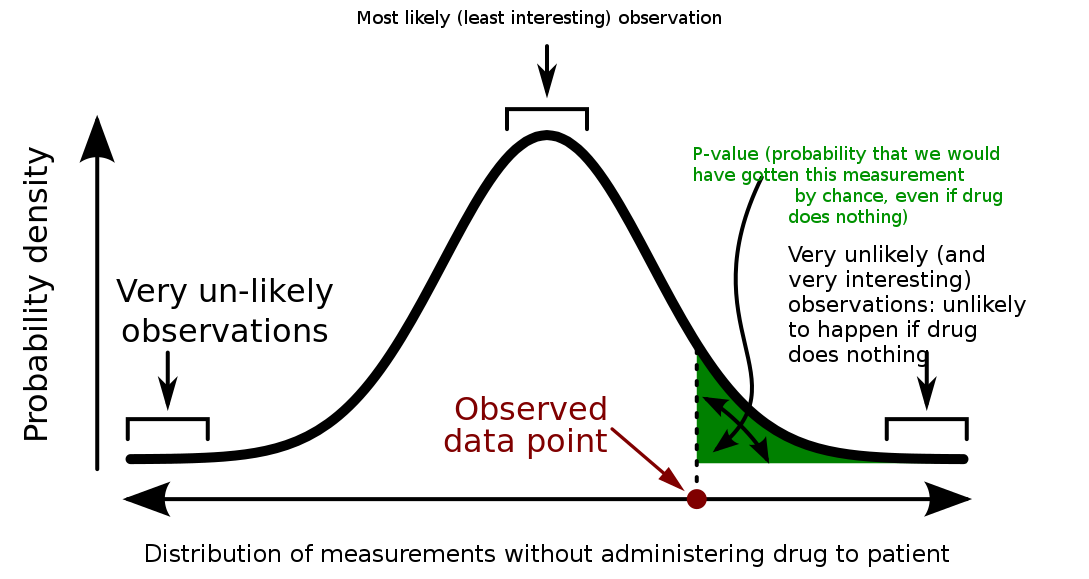
\includegraphics[width=0.8\textwidth]{gaussian.png}
%\EC
%}
%
%\frame{\frametitle{\textbf{Statistical inference gone wrong, II: biased data}}
%
%\BS
%
%Biased data (the survivorship bias from Exam 2 is an example):
%\BI
%\item Make lots of measurements of how people react to the drug
%\item {\color{Red} Fail to measure the ones on the left-hand side (they're dead)}
%\item Compare their distribution to the black curve (what you'd expect if the drug does nothing)
%\item {\color{Red} We removed the left-hand side, so the average shifts right}
%\item {\color{Red} Notice that their average is very different, get excited!}
%\EI
%
%
%\BC
%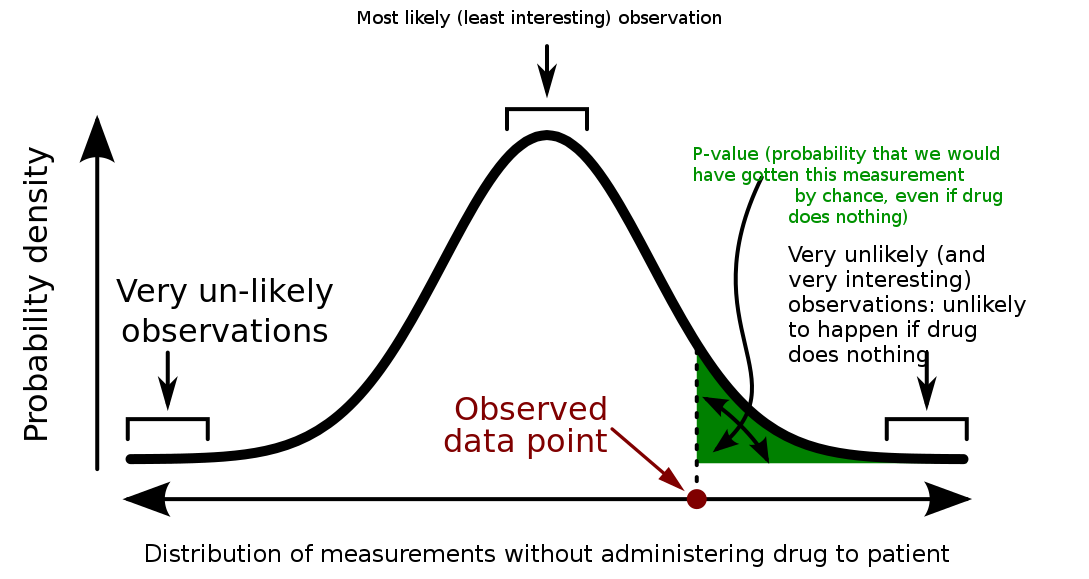
\includegraphics[width=0.8\textwidth]{gaussian.png}
%\EC
%}
%
%\frame{\frametitle{\textbf{Statistical inference gone wrong, III: publication bias}}
%
%\BS
%
%If the measurements are entire {\it studies}, we often unintentionally cherry-pick them in {\it meta-analyses} (studies 
%averaging many studies together)
%\BI
%\item Different scientists do experiments on how people react to the drug
%\item {\color{Red} Nobody publishes the ones close to the center (they're boring, back to the drawing board!) }
%\item Compare their distribution to the black curve (what you'd expect if the drug does nothing)
%\item {\color{Red} Even if the drug does nothing, you'll get a distribution looking like the green portion}
%\item {\color{Red} Notice that their average is very different, get excited!}
%\EI
%
%
%\BC
%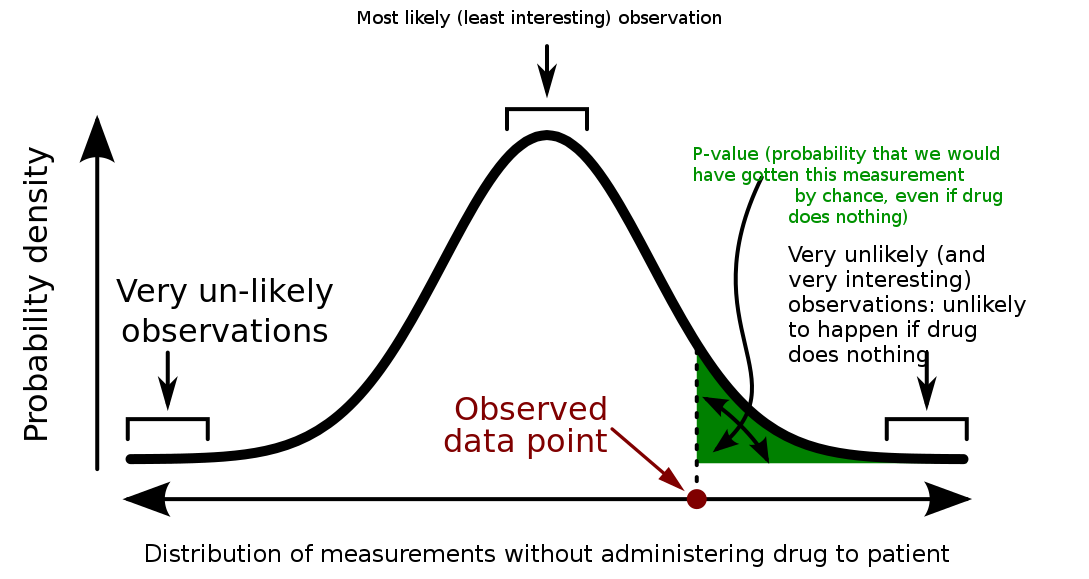
\includegraphics[width=0.8\textwidth]{gaussian.png}
%\EC
%}
%
%\frame{
%
%\Large
%\BC
%Do you have any favorite examples of statistical shenanigans being used to support flawed claims?
%
%\BS
%
%(Post to Slack for extra credit)
%\large
%\EC
%
%\BS\pause
%\BS
%The above example about drug studies is real: publication bias is a serious problem in drug 
%development! (See \url{https://www.nejm.org/doi/full/10.1056/NEJMsa065779})
%}
%
%\frame{\frametitle{\textbf{Unit 4: rotational dynamics}}
%
%\Large
%
%In the last unit we studied momentum and kinetic energy, along with their rotational counterparts:
%
%\BCC
%
%\HC
%\color{Blue}
%\BC
%\Large
%Translation
%\large
%
%Momentum $\vec p = m \vec v$
%
%Kinetic energy $KE = \frac{1}{2}mv^2$
%\EC
%
%\HC
%\color{Red}
%\BC
%\Large
%Rotation
%\large
%
%Angular momentum $L = I \omega$
%
%Kinetic energy $KE_{\rm rot} = \frac{1}{2}I\omega^2$
%\EC
%
%\ECC
%
%\BS\BS
%
%This already suggests some other correspondences between translational and rotational quantities:
%
%\BI
%\item Velocity $\Longleftrightarrow$ Angular velocity
%\item Mass $\Longleftrightarrow$ Moment of inertia
%\EI
%
%Are there others like this? In what other ways does rotational motion have familiar features?
%
%}

\frame{\frametitle{\textbf{Announcements}}
	\large
	\BI
	\item Homework 8 is due Friday in recitation. It consists of a redo of Exam 3, along with one other problem
	\item See the ``second chance'' section of the website for specific tutorial times
	\item I'll also be in the Physics Clinic today from 4-5pm offering general help to people
	\EI
	

}
	
	
	


\frame{\frametitle{\textbf{Unit 4: rotational dynamics}}

\large

As we saw last time, {\it almost all of what we have done already} works just the same for rotation.

\BS

Last time we saw an example: {\it \color{Green} rotational kinetic energy}. A summary:


\begin{center}
	\color{Red} A rotating object has rotational kinetic energy {\color{Green}${\rm{KE}}_{rot} = \frac{1}{2}I \omega^2$.}
\end{center}

\pause

\BI
\item $I$ is the moment of inertia -- the rotational equivalent of mass
\item $\omega$ is the object's angular velocity -- the rotational equivalent of velocity
\item An object that is rolling without slipping both moves {\it and} translates -- we'll return to this
\EI

\BS\BS\pause

The moral:

\BI
\item {\color{Blue}Rotational motion works much like translational motion}
\item {\color{Red}... but there are sometimes a few extra things to think about.}
\EI

\BS

This is just a slice of rotational motion. Now let's look from the ground up, starting from the beginning!
}



\frame{\frametitle{\textbf{Unit 4: rotational dynamics}}

\BS

Unit 1:
\BI
\item The kinematics relations between $\vec a, \vec v, \vec s, t$ are identical for $\alpha, \omega, \theta, t$
\item They're even simpler, because there are no vectors!
\EI

\BS
\BS

Unit 2:
\BI
\item The centerpiece of this course was $\vec F = m \vec a$: ``how do forces make things move?''
\item {\color{Red}What is the rotational analogue to this?}
\EI

\BS\BS

Now we will:

\BI
\item Learn the rotational analogue of {\color{Red} force} and {\color{Red} Newton's second law} (today)
\item Apply it to all sorts of situations: the rest of the term!
\EI

\BS

First, let's look again at the whole picture of how rotational and translational motion correspond:
}

\frame{
\begin{center}
\begin{tabular}{l | l}

 \multicolumn{1}{c|}{\Large Translation} & \multicolumn{1}{c}{\Large Rotation} \\
 \\
\hline
\hline
 & \\
Position $\vec s$ & Angle $\theta$ \\
Velocity $\vec v$ & Angular velocity $\omega$ \\
Acceleration $\vec a$ & Angular acceleration $\alpha$ \\
 & \\
\hline
\hline
 & \\
Kinematics: $\vec s(t)=\frac{1}{2}\vec at^2 + \vec v_0 t + \vec s_0$ & $\theta(t) = \frac{1}{2}\alpha t^2 + \omega_0 t + \theta_0$ \\
 & \\
\hline
\hline

 & \\
Force $\vec F$ & Torque $\tau$ \\
Mass $m$ & Rotational inertia $I$ \\
Newton's second law $\vec F = m \vec a$ & Newton's second law for rotation $\tau = I \alpha$ \\
 & \\

\hline
\hline

 & \\
Kinetic energy $KE=\frac{1}{2}mv^2$ & Kinetic energy $KE=\frac{1}{2}I\omega^2$ \\
Work $W = \vec F \cdot \Delta \vec s$ & Work $W = \tau \Delta \theta$ \\
Power $P = \vec F \cdot \vec v$ & Power $P = \tau \omega$ \\
 & \\

\hline
\hline

 & \\
Momentum $\vec p = m \vec v$ & Angular momentum $L = I\omega$\\
 & \\

\hline
\end{tabular}
\end{center}
}



\frame{
\begin{center}
\begin{tabular}{l | l}

 \multicolumn{1}{c|}{\Large Translation} & \multicolumn{1}{c}{\Large Rotation} \\
 \\
\hline
\hline
 & \\
\color{Red} Position $\vec s$ & \color{Red} Angle $\theta$ \\
\color{Red} Velocity $\vec v$ & \color{Red} Angular velocity $\omega$ \\
\color{Red} Acceleration $\vec a$ & \color{Red} Angular acceleration $\alpha$ \\
 & \\
\hline
\hline
 & \\
\color{Red} Kinematics: $\vec s(t)=\frac{1}{2}\vec at^2 + \vec v_0 t + \vec s_0$ & \color{Red} $\theta(t) = \frac{1}{2}\alpha t^2 + \omega_0 t + \theta_0$ \\
 & \\
\hline
\hline
 & \\
Force $\vec F$ & Torque $\tau$ \\
Mass $m$ & Rotational inertia $I$ \\
Newton's second law $\vec F = m \vec a$ & Newton's second law for rotation $\tau = I \alpha$ \\
 & \\

\hline
\hline

 & \\
Kinetic energy $KE=\frac{1}{2}mv^2$ & Kinetic energy $KE=\frac{1}{2}I\omega^2$ \\
Work $W = \vec F \cdot \Delta \vec s$ & Work $W = \tau \Delta \theta$ \\
Power $P = \vec F \cdot \vec v$ & Power $P = \tau \omega$ \\
 & \\

\hline
\hline

 & \\
Momentum $\vec p = m \vec v$ & Angular momentum $L = I\omega$\\
 & \\

\hline
\end{tabular}
\end{center}
}
%
%\frame{
%\begin{center}
%\begin{tabular}{l | l}
%
% \multicolumn{1}{c|}{\Large Translation} & \multicolumn{1}{c}{\Large Rotation} \\
% \\
%\hline
%\hline
% & \\
%Position $\vec s$ & Angle $\theta$ \\
%Velocity $\vec v$ & Angular velocity $\omega$ \\
%Acceleration $\vec a$ & Angular acceleration $\alpha$ \\
% & \\
%\hline
%\hline
% & \\
%Kinematics: $\vec s(t)\frac{1}{2}\vec at^2 + \vec v_0 t + \vec s_0$ & $\theta(t) = \frac{1}{2}\alpha t^2 + \omega_0 t + \theta_0$ \\
% & \\
%\hline
%\hline
%
% & \\
%Force $\vec F$ & Torque $\tau$ \\
%Mass $m$ & Rotational inertia $I$ \\
%Newton's second law $\vec F = m \vec a$ & Newton's second law for rotation $\tau = I \alpha$ \\
% & \\
%
%\hline
%\hline
%
% & \\
%\color{Red}Kinetic energy $KE=\frac{1}{2}mv^2$ & \color{Red}Kinetic energy $KE=\frac{1}{2}I\omega^2$ \\
%Work $W = \vec F \cdot \Delta \vec s$ & Work $W = \tau \Delta \theta$ \\
%Power $P = \vec F \cdot \vec v$ & Power $P = \tau \omega$ \\
% & \\
%
%\hline
%\hline
%
% & \\
%\color{Red}Momentum $\vec p = m \vec v$ & \color{Red}Angular momentum $L = I\omega$\\
% & \\
%
%\hline
%\end{tabular}
%\end{center}
%}

\frame{
\begin{center}
\begin{tabular}{l | l}

 \multicolumn{1}{c|}{\Large Translation} & \multicolumn{1}{c}{\Large Rotation} \\
 \\
\hline
\hline
 & \\
\color{Grey}Position $\vec s$ & \color{Grey}Angle $\theta$ \\
\color{Grey}Velocity $\vec v$ & \color{Grey}Angular velocity $\omega$ \\
\color{Grey}Acceleration $\vec a$ & \color{Grey}Angular acceleration $\alpha$ \\
 & \\
\hline
\hline
 & \\
\color{Grey}Kinematics: $\vec s(t)=\frac{1}{2}\vec at^2 + \vec v_0 t + \vec s_0$ & \color{Grey}$\theta(t) = \frac{1}{2}\alpha t^2 + \omega_0 t + \theta_0$ \\
 & \\
\hline
\hline

 & \\
\color{Red}Force $\vec F$ & \color{Red}Torque $\tau$ \\
\color{Green}Mass $m$ & \color{Green}Rotational inertia $I$ \\
\color{Green}Newton's second law $\vec F = m \vec a$ & \color{Green}Newton's second law for rotation $\tau = I \alpha$ \\
 & \\

\hline
\hline

 & \\
\color{Grey}Kinetic energy $KE=\frac{1}{2}mv^2$ & \color{Grey}Kinetic energy $KE=\frac{1}{2}I\omega^2$ \\
\color{Grey}Work $W = \vec F \cdot \Delta \vec s$ & \color{Grey}Work $W = \tau \Delta \theta$ \\
\color{Grey}Power $P = \vec F \cdot \vec v$ & \color{Grey}Power $P = \tau \omega$ \\
 & \\

\hline
\hline

 & \\
\color{Grey}Momentum $\vec p = m \vec v$ & \color{Grey}Angular momentum $L = I\omega$\\
 & \\

\hline
\end{tabular}
\end{center}
}


\frame{\frametitle{\textbf{Rotational motion and kinematics}}
\large
A reminder about describing rotational motion:

\normalsize

\BI
\item Instead of describing the change in an object's position $\vec s$, we describe the change in its angle $\theta$
\item Velocity $\vec v \rightarrow$ angular velocity $\omega$ (we've used this often before)
\item {\color{Red}Acceleration $\vec a \rightarrow$ angular acceleration $\alpha$}
\EI

All the kinematics you learned carries over. For instance:

$$\theta(t) = \frac{1}{2}\alpha t^2 + \omega_0 t + \theta_0$$

\pause\BS\BS

\begin{center}
	Now the question: what makes objects rotate in the first place?
\end{center}


}

\frame{\frametitle{\textbf{What corresponds to Newton's second law?}}
  \Large
  \centerline{The key idea in translational motion is Newton's second law $\vec F = m \vec a$.}


  \bigskip
  \bigskip

  \pause

  \centerline{What is the corresponding idea for rotational motion?}

\bigskip
\bigskip

  \BI
\item{Angular acceleration $\alpha$ corresponds to $\vec a$}

\item{The rotational analogue of mass is called {\bf \color{Red} moment of inertia $I$} (you already know this)}
\item{The rotational analogue of force is called {\bf \color{Red} torque $\tau$} \\ (we need to understand what this is today!)}
  \EI
  \bigskip
  \bigskip


 % \centerline{Today, we'll study only torque: this limits us to situations where $\alpha=0$.}

}

\frame{\frametitle{\textbf{Torque}}
  \Large
  \centerline{Torque ($\tau$) is the rotational analogue of force: ``rotational push or pull''}

  \BI
  \large
\item{Forces applied to an object result in torques: ``push on something to turn it''}
\item{The size of the torque depends on three things:}
  \pause
\item{The size of the force}
  \BI
\item{Push harder to exert more torque -- that's easy!}
  \EI
  \pause\BS
\item{The distance from the force to the pivot point}
  \BI
\item{The further from the pivot to the point of force, the greater the torque}
\item{This is why the door handle is on the outside of the door...}
  \EI
  \BS\pause
\item{The angle at which the force is applied}
  \BI
\item{Only forces ``in the direction of rotation'' make something turn}
\item{The torque depends only on the {\it component of the force perpendicular to the radius}}
  \EI
  \EI
}


\frame{\frametitle{\textbf{Computing torque}}
  \centerline{\Huge $\tau = F_\perp r$}
\begin{center}
\Large Torque is equal to the distance from the pivot, \\times the perpendicular component of the force
\end{center}


\bigskip
  \centerline{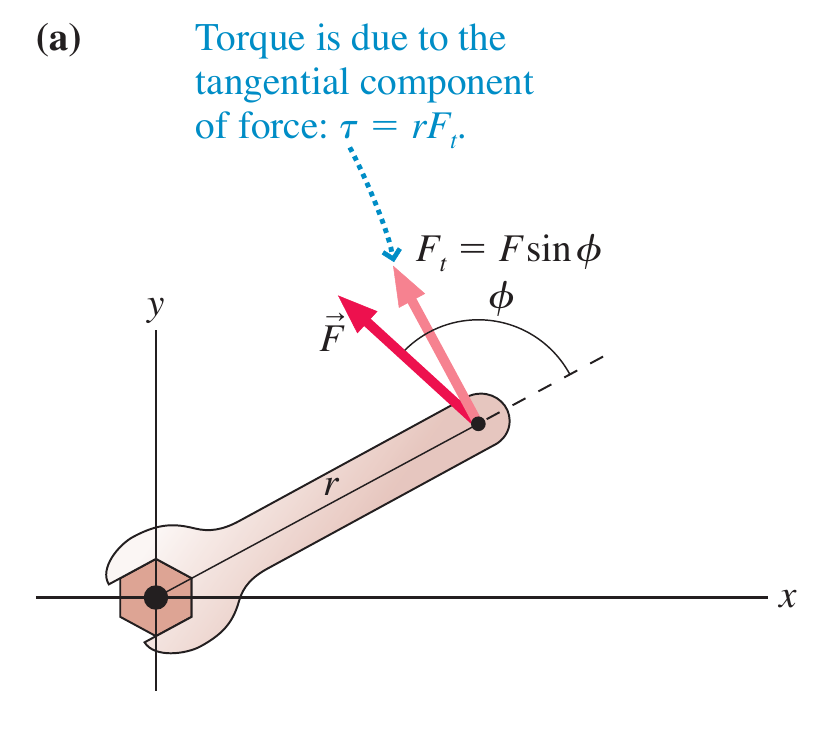
\includegraphics[width=0.3\textwidth]{torque1.png}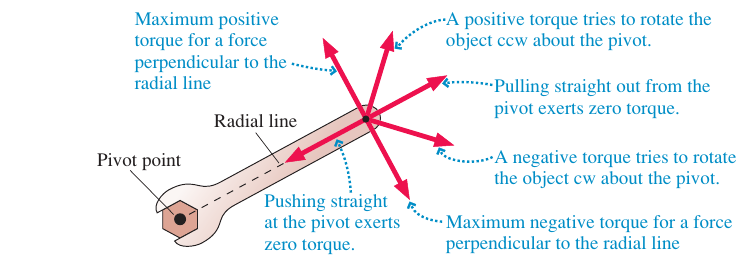
\includegraphics[width=0.6\textwidth]{torque2.png}}

\bigskip

  \centerline{Note that torque has a sign, just like angular velocity: CCW is positive; CW is negative.}
}

\frame{\frametitle{\textbf{Computing torque}}
\BI
\item{We can think of the torque in any other equivalent way; there is another one that's often useful}
\item{The previous way: {\bf \color{Red}``The radius vector, times the component of force perpendicular to it''}}
\item{The alternative: {\bf \color{Green}``The force vector, times the component of the radius perpendicular to it''}}
\EI
\centerline{\large{Here's the figure from the text:}}
\centerline{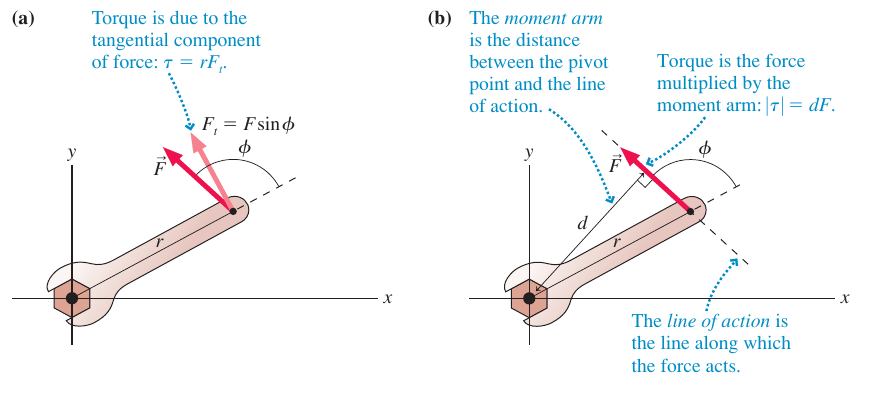
\includegraphics[width=0.6\textwidth]{momentarm.png}}
\bigskip
%\centerline{I'll draw a clearer version on the document camera}
}

\frame{
\Large

\BC
Which bar is hardest to hold up? (See document camera)
\EC


}



\frame{\frametitle{\textbf{Important notes about torque}}
  \centerline{\Large These are very important: note them somewhere for later reference!}
  \bigskip
  \bigskip
  \BI
\item{Torques are in reference to a {\bf particular pivot}}
\item{This is different from force; if you're talking about torque, you {\it must} say what axis it's measured around}
\item{Torque now depends on the {\it location} of forces, not just their size}
\BI
\item{Your force diagrams now need to show the place where forces act!}
\item{Weight acts at the center of mass (``the middle''); we'll see what that means later}
\item{A sample force diagram might look like this:}

  \bigskip

  \centerline{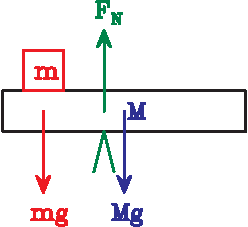
\includegraphics[width=0.3\textwidth]{diag-crop.pdf}}
  \EI
\EI
  }
\frame{\frametitle{\textbf{Drawing diagrams: torque problems}}
\large
\BI
\item{Now you need to draw the position at which every force acts}
\item This is called an ``extended force diagram''
\item{Pick a pivot; label it: remember torques must be calculated around that pivot}
\BS\BS\pause
\item{Remember, the torque from each force is either...}
\BI
\item{\color{Red}$F_\perp r$ (most useful)}
\item{\color{Blue}$F r_\perp$ (sometimes useful)}
\item{\color{Green}$F r \sin \theta$ ($\theta$ is angle between vectors)}
\item{Direction of torques matters!}
\EI
\EI
}

\frame{\frametitle{\textbf{Equilibrium problems}}
\Large
\BI
\item{Often we know $\alpha = \vec a = 0$}
\item{This tells us that the net torque (about {\it any} pivot) and the net force are both zero}
\item{Usually this is because an object isn't moving, but sometimes it's moving at a constant rate}
\BS\color{Red}

\item{Compute the torque about any point and set it to zero}
\item{Choose a pivot at the location of a force we don't care about so its torque is zero}
\item{If needed, also write $\sum \vec F = 0$}
\EI
}

\frame{\frametitle{\textbf{Statics problems: a sample}}
\large
\BI
\item{What is the weight of the bar?}
\pause
\item{How does the force needed to support it depend on the angle of the force?}
\pause
\item{How does the force needed to support it depend on the angle of the bar?}
\pause
\item{What if I hang weights from it?}
\EI
}


\end{document}
